\documentclass[../main/thesis]{subfiles}

\begin{document}

\section{Model development log and notes}
% The intention of this section is currently to log the notes made during model development. What is written may be discussion like, and can thus be used as a basis for the actual thesis. However, this section is to be included in the final thesis.tex after extensive rewriting. Remember that good thesis work is well documented thesis work!
\subsection{Two day forecast}
Data sources used are Sea Ice charts from Nick initiated at 15:00 as well as Arome Arctic initiated at 18:00 \cite{MOI2015,Mueller2017}. For a given date, the current Ice Chart is used as a predictor for the model, while the Ice Chart drawn two days later is supplied as the model target. Moreover, the Arome Arctic data is structured such that the period between lead time 0 - 18 and 18 - 42 is stored as mean products. Thus, the period covering lead hours 3 - 21 and 21 - 45 relative to the Ice Charts are covered (and meaned). The 4d variables used from AA (which feature a temporal dimension) are T2M, Xwind and Ywind, the 3d variable used is SST, which is available in the data, though the variable itself is only utilized to force the Data Assimilation system of AA and not a product of the prediction system. Finally, a land sea mask present on previously available ice charts on lustre is adopted to fit the current data, and is used both as a predictor as well as a mask when computing metrics and visualizing results.

The model developed for the two day prediction is based on the SimpleUNET architecture, though with a different sized Input layer to accommodate for the changed dataloader. The dataloader has subsequently been changed to appropriately select the correct fields from the .hdf5 samples and appoint them as input or target variables. As a result of using three variables of two days mean AA forecast, as well as sst, land-sea-mask and current time-step ice chart, the total number of predictors fed into the model is 9. Moreover, the resolution of all fields are kept at 1km, though their spatial extent is limited to (1920 x 1840). This resolution and spatial size conserves (almost) the entirety of the west-east axis of the AA domain. However, the southern border is raised by 450km compared to the AA domain. There are two main motivations behind readjusting the spatial extent of the predictors and targets.

\begin{itemize}
    \item[1.] The spatial extent of the input domain has to be divisible by the reducing factor enforced by the MaxPooling operation performed in the encoding component of the UNET.
    \item[2.] The southern latitudes covered by AA has a proportionally skewed Sea Ice / Ice Free open water ratio, as exemplified in Figure (\ref{fig:exampleAAsouthborder}). Increasing the southern bounding latitude of the subdomain thus decreases the number of guaranteed ice free pixels, which in turn decreases the skewness towards the ice free open water class for the UNET.
\end{itemize}

\begin{figure}
    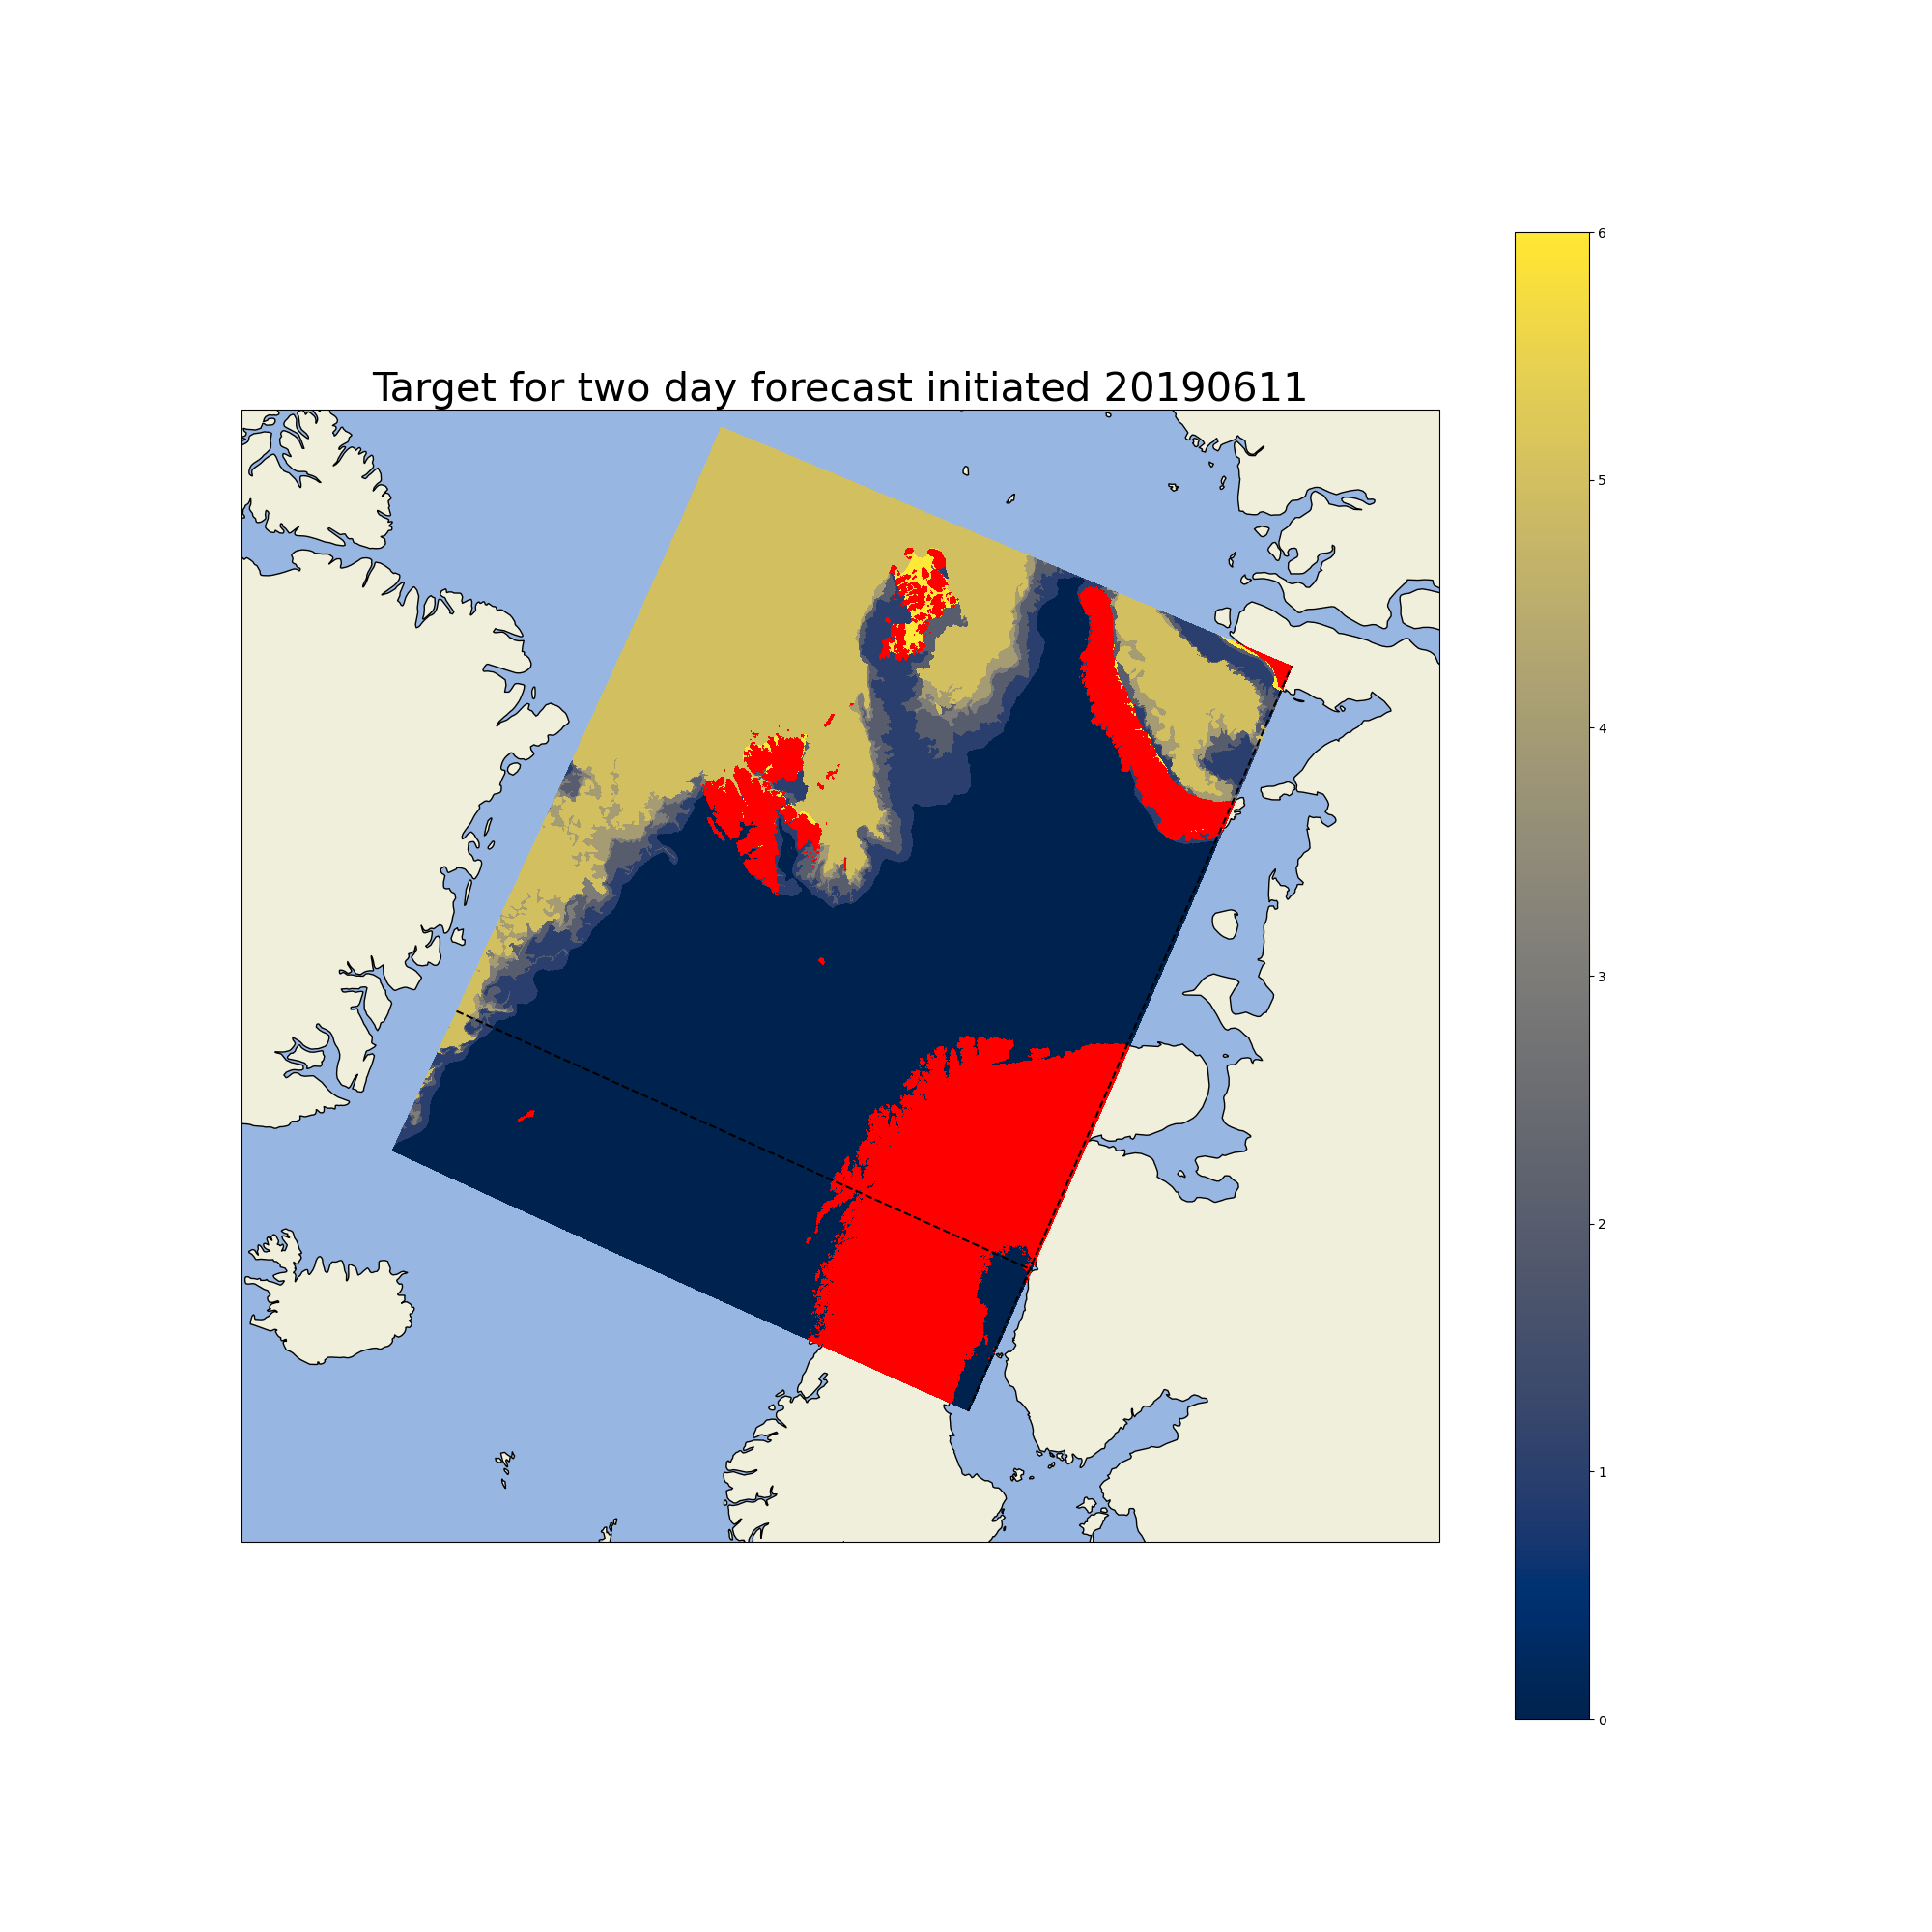
\includegraphics[trim={0 10cm 11cm 9cm}, clip, width=\textwidth]{/home/arefk/uio/MScThesis_AreKvanum2022_SeaIceML/thesis/model_development/figures/20190611.png}
    \caption{\label{fig:exampleAAsouthborder}Example sample displaying an Ice Chart on a 1km Arome Arctic projection. Note the horizontal and vertical dashed black line which indicate the domain subsection used by the UNET}
\end{figure}

\subsection{Model Architecture}
The model architecture follows an encoder - decoder structure, commonly referred to as a U-NET \cite{Ronneberger2015} due to its shape funnelling the spatial data to coarser resolution, which resembles the letter "U". The current U-NET implementation follows that of Ronneberger et.al, though it has been modified with batch normalization after each convolution operation to ensure a more stable gradient flow. The weights of the model are Kaiming-He initialized \cite{He2015}, as the activation function used throughout the network is the ReLU function \cite{Nair2010}. The final output of the model is a (1920, 1840, 7) tensor containing softmaxed probabilities along its final axis.

\subsection{CategoricalCrossEntropy-Loss}
As the title suggests, these runs of the model involved using CategoricalCrossEntropy as the loss function for multi-class image segmentation. Categorical Cross Entropy loss is defined as 

\begin{equation}
    \label{eq:CE}
    CE = - \sum_i^C y_i\log{(\hat{y_i})}
\end{equation}

where $C$ denotes the number of available classes, $y$ the ground truth and $\hat{y}$ a prediction of $y$. Note that as $y$ is onehot-encoded, the formulated function only contributes to the overall loss with the log of the predicted probability of the correct class according to the ground truth.

Two variants of the previously described model have been trained with the CategoricalCrossEntropy described in equation (\ref{eq:CE}). The first model was trained with an encoder consisting of 4 convolutional blocks with channel dimensions (64, 128, 256, 512). The second model consisted of 5 convolutional blocks, with an identical architecture except for the last convolutional block increasing the channel dimension to (1024). Example outputs as well as target can be seen in Figure (\ref{fig:20210611}).

\begin{figure}
    \begin{subfigure}{0.49\textwidth}
        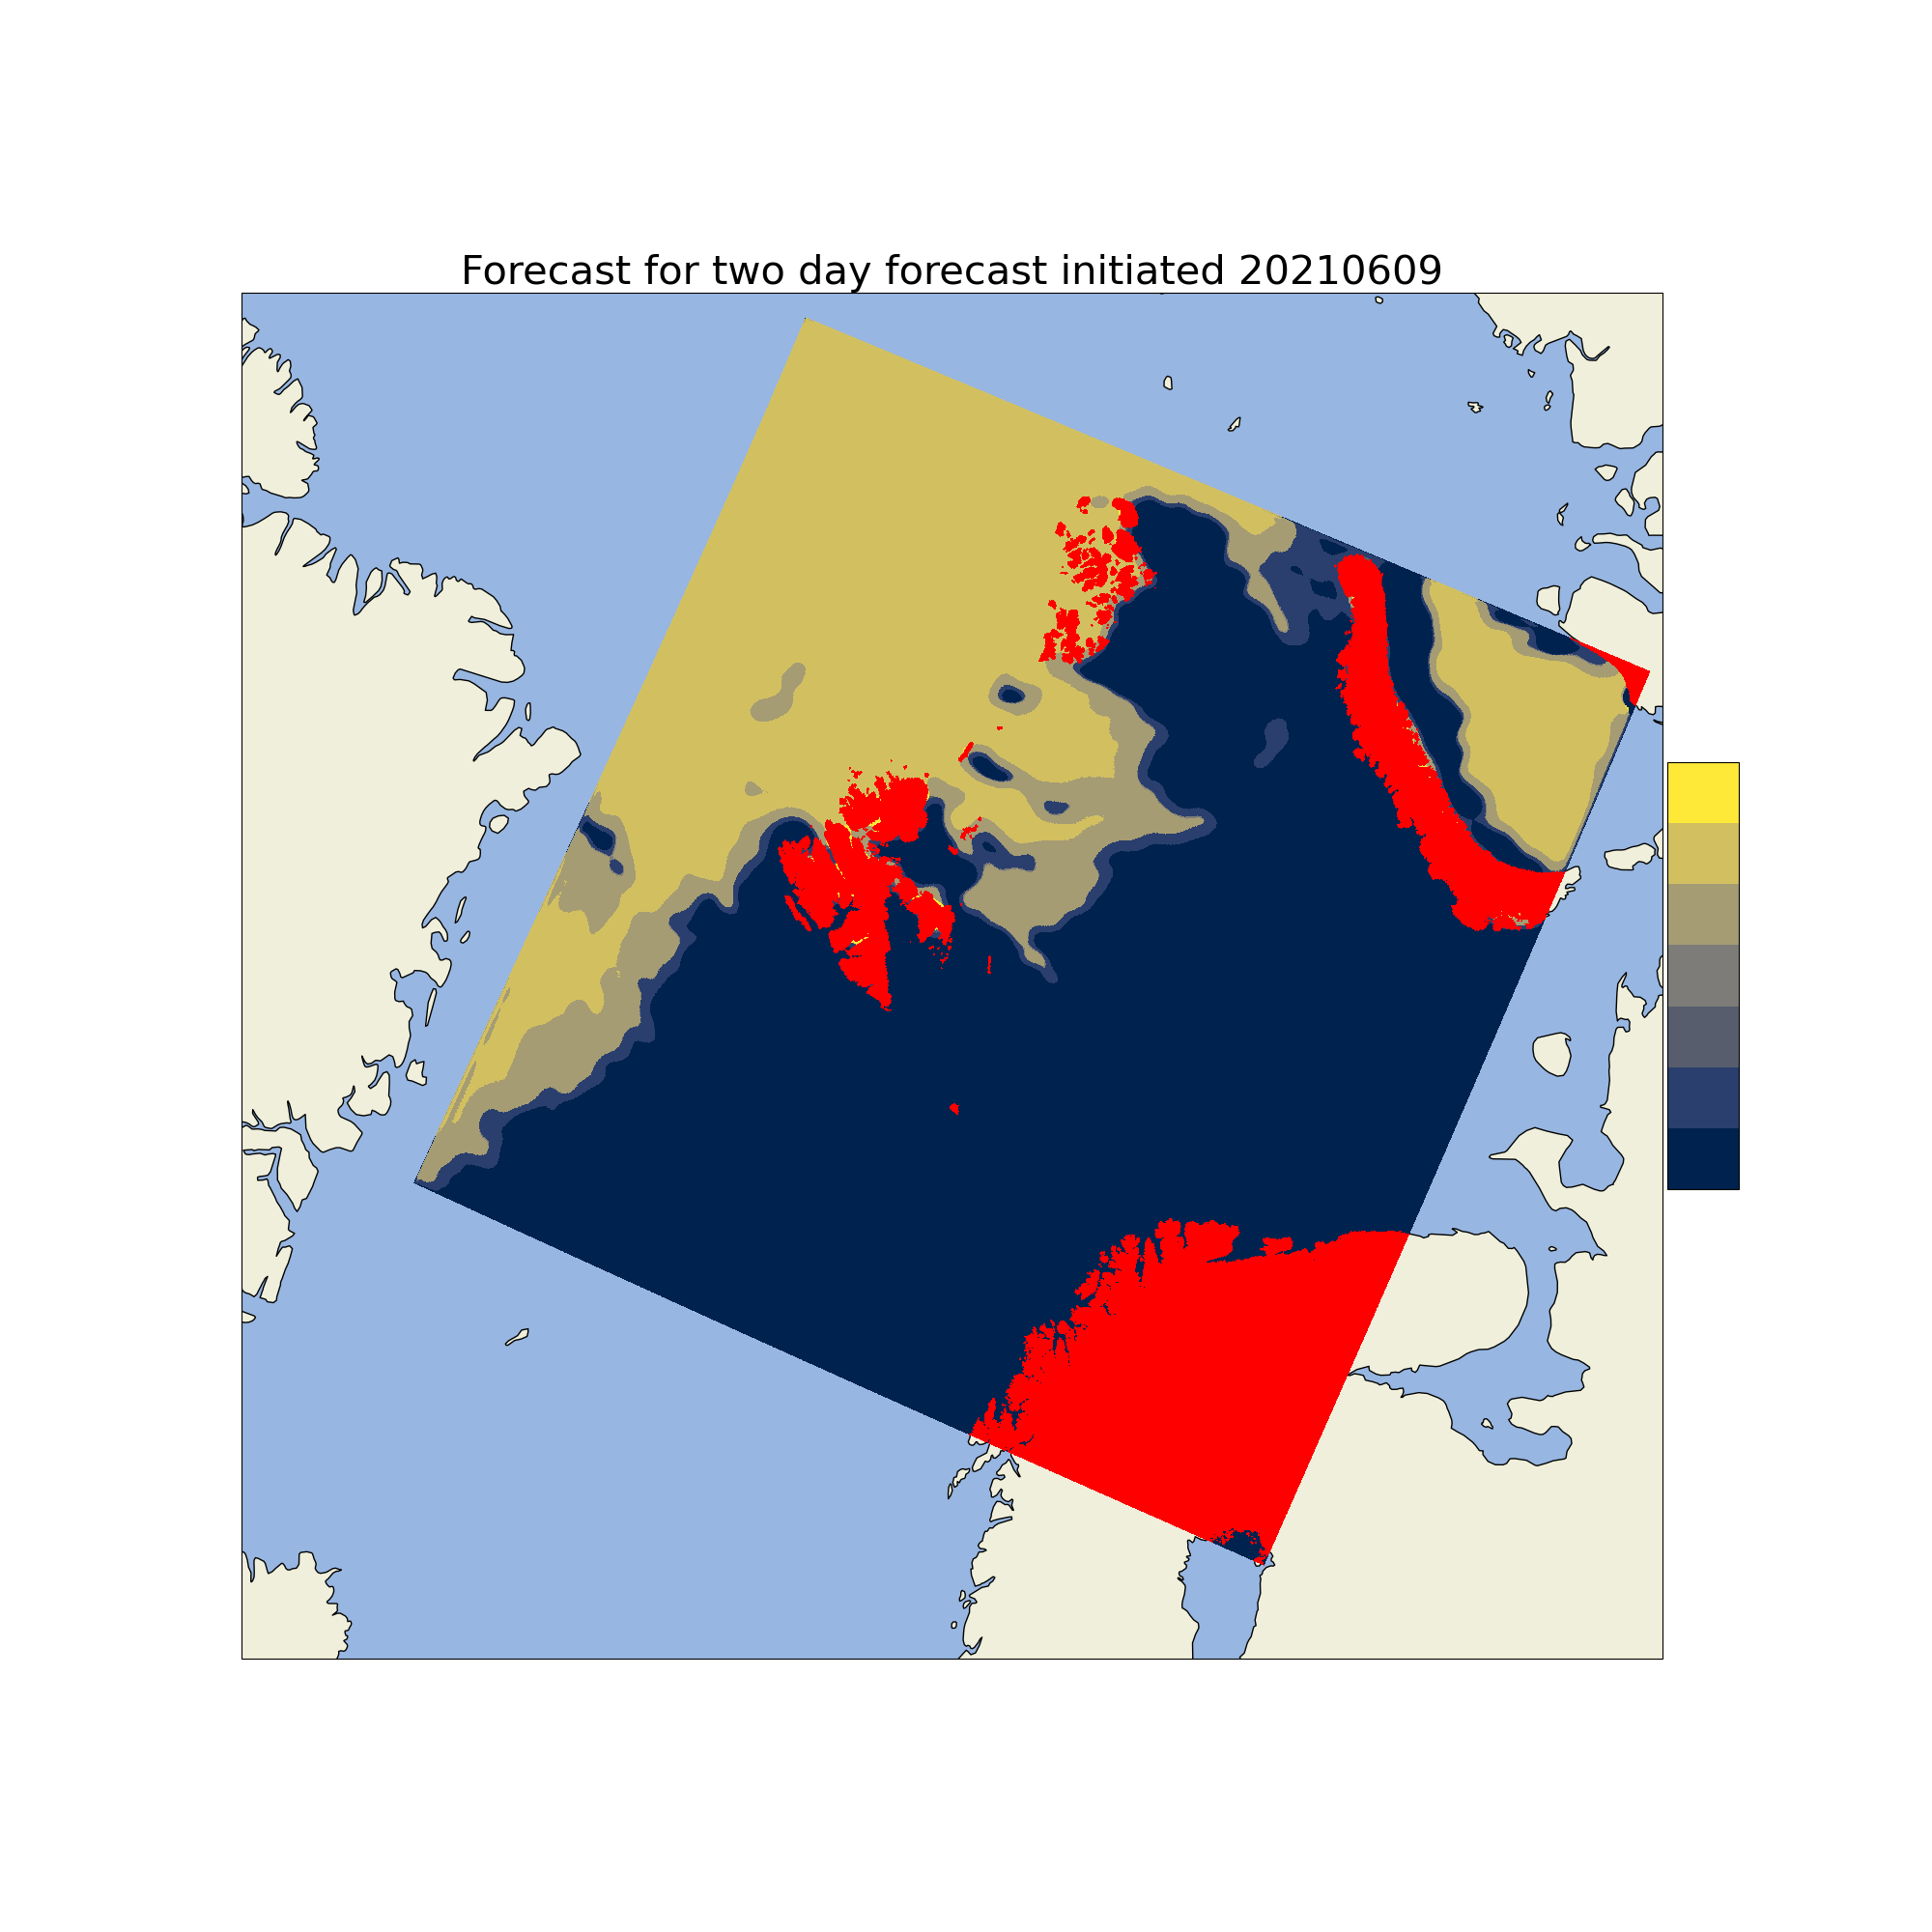
\includegraphics[width=\textwidth]{/home/arefk/uio/MScThesis_AreKvanum2022_SeaIceML/thesis/model_development/figures/20210611_512.png}
        \caption{\label{fig:model51220210611}Forecast with two day lead time with model\_512 architecture}
    \end{subfigure}
    \hfill
    \begin{subfigure}{0.49\textwidth}
        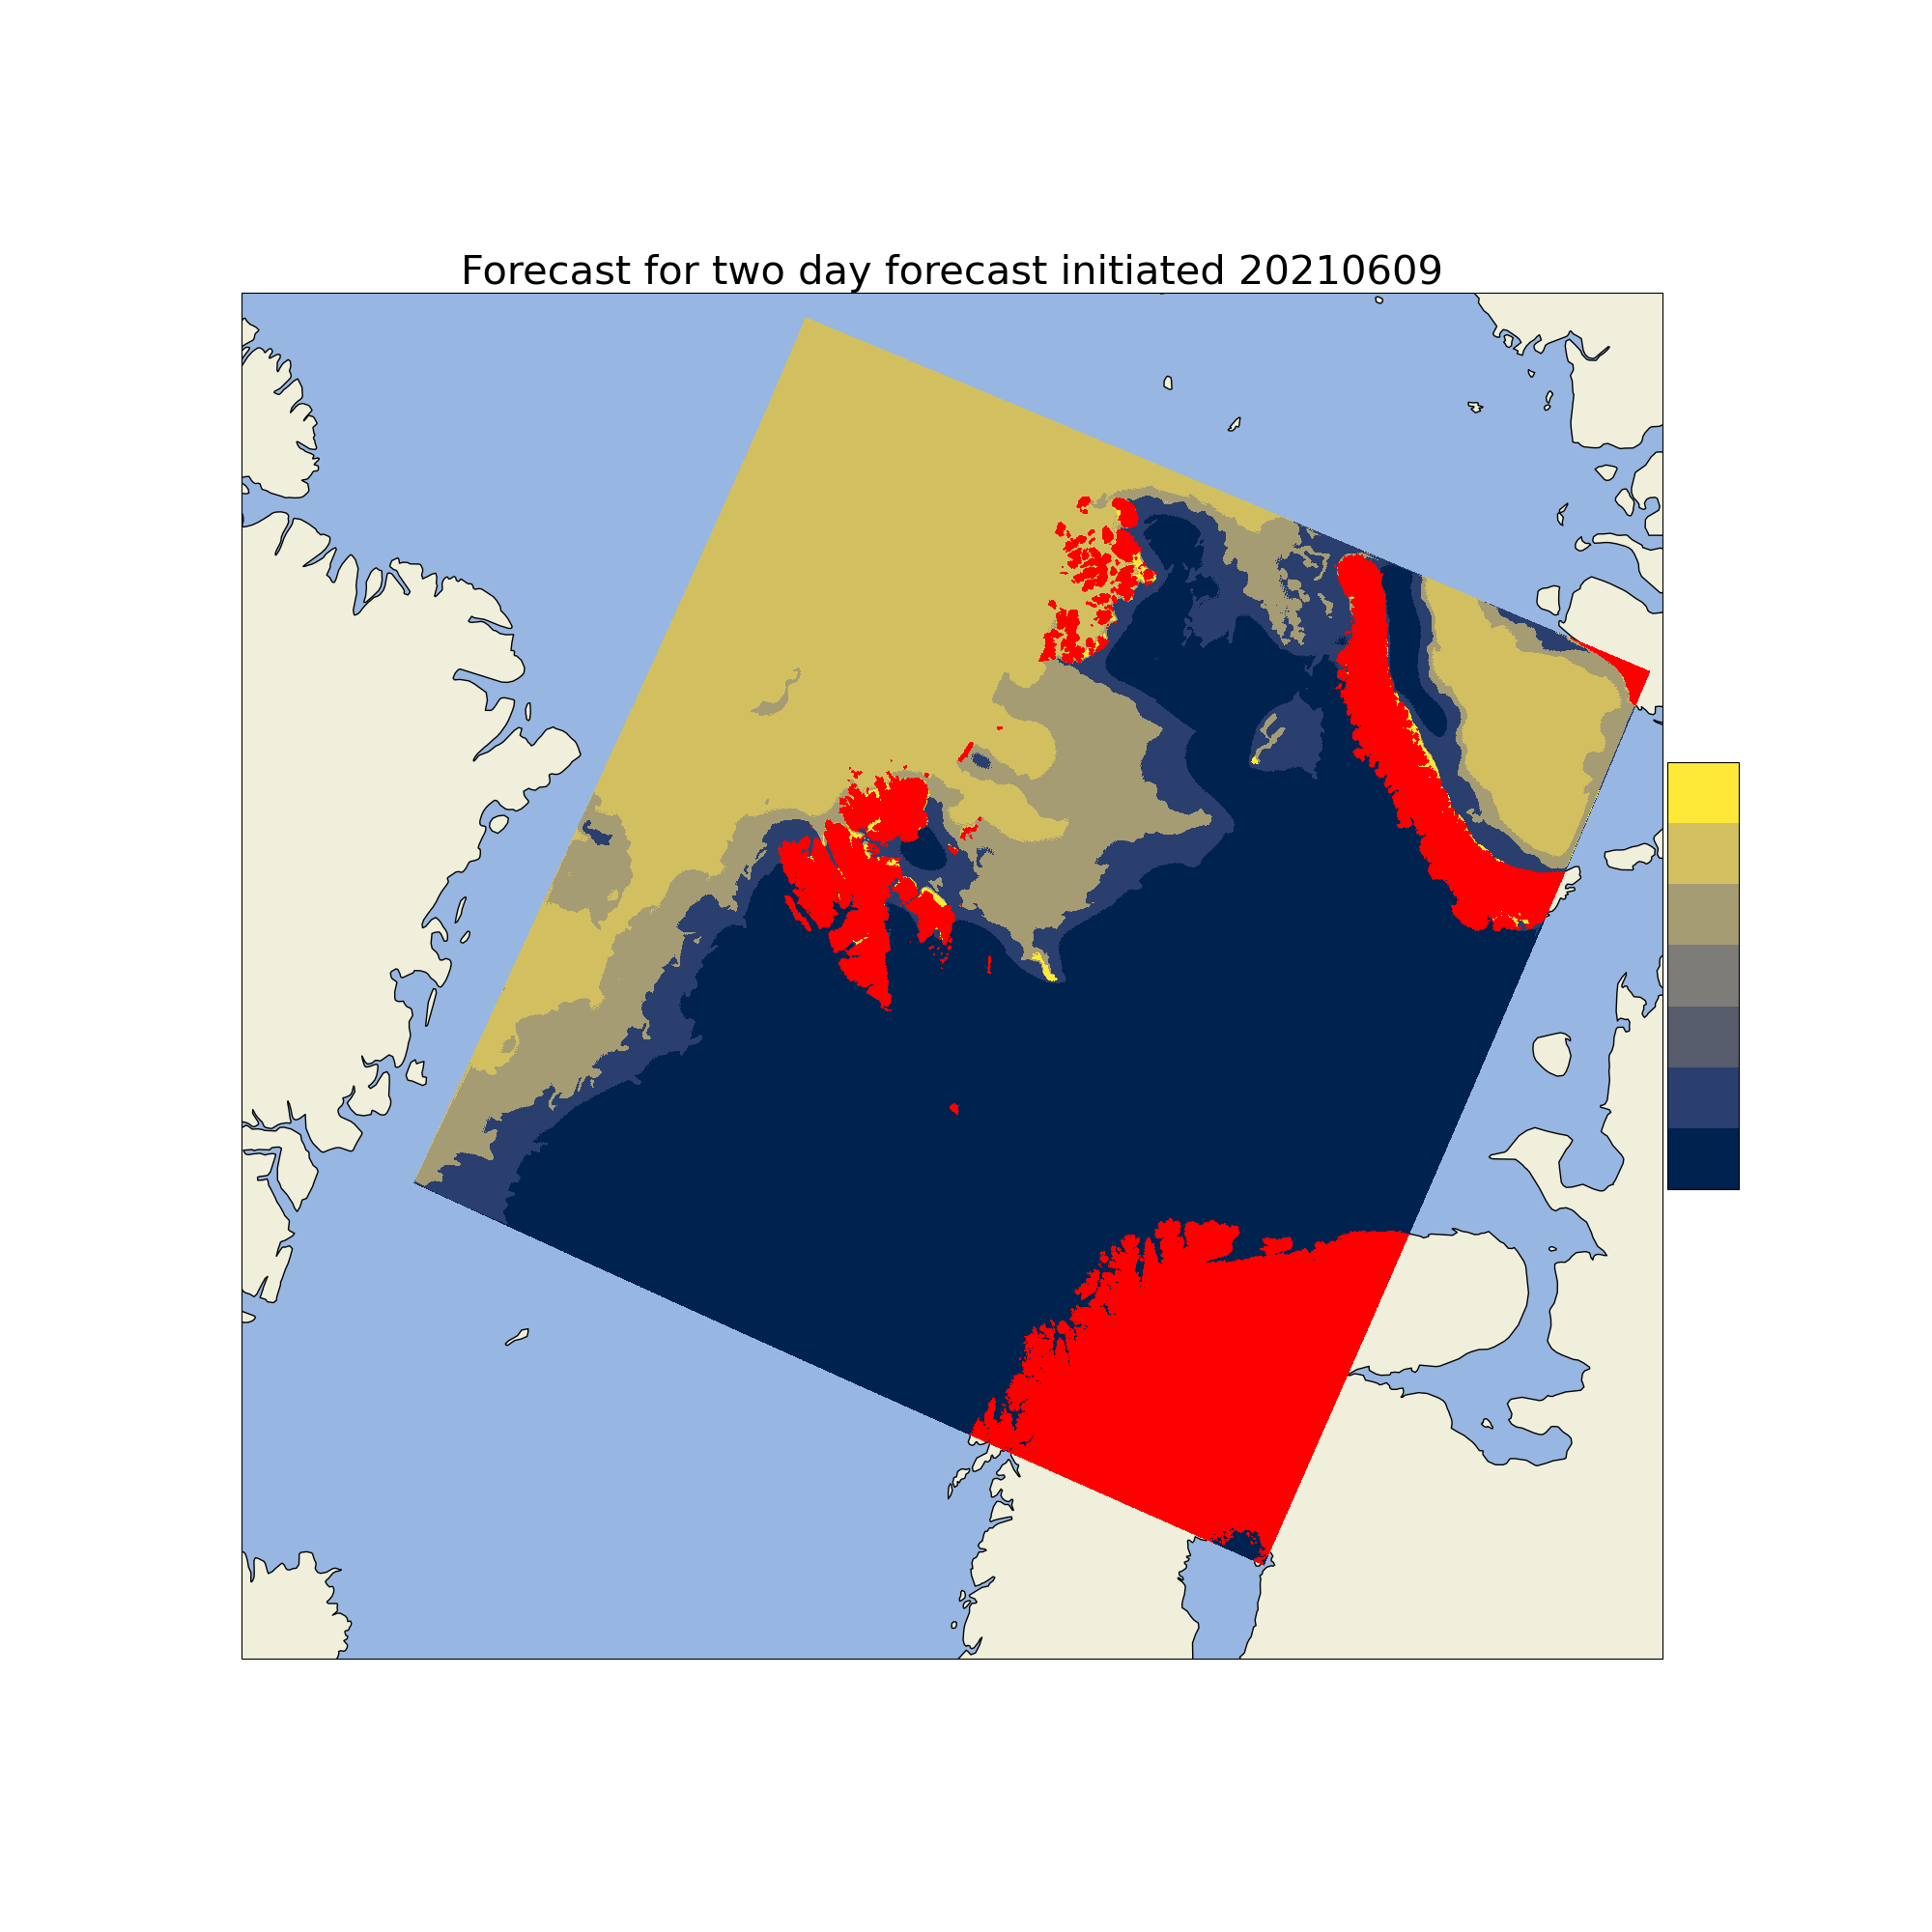
\includegraphics[width=\textwidth]{/home/arefk/uio/MScThesis_AreKvanum2022_SeaIceML/thesis/model_development/figures/20210611_1024.png}
        \caption{\label{fig:model102420210611}Forecast with two day lead time with model\_1024 architecture}
    \end{subfigure}
    \begin{subfigure}{\textwidth}
        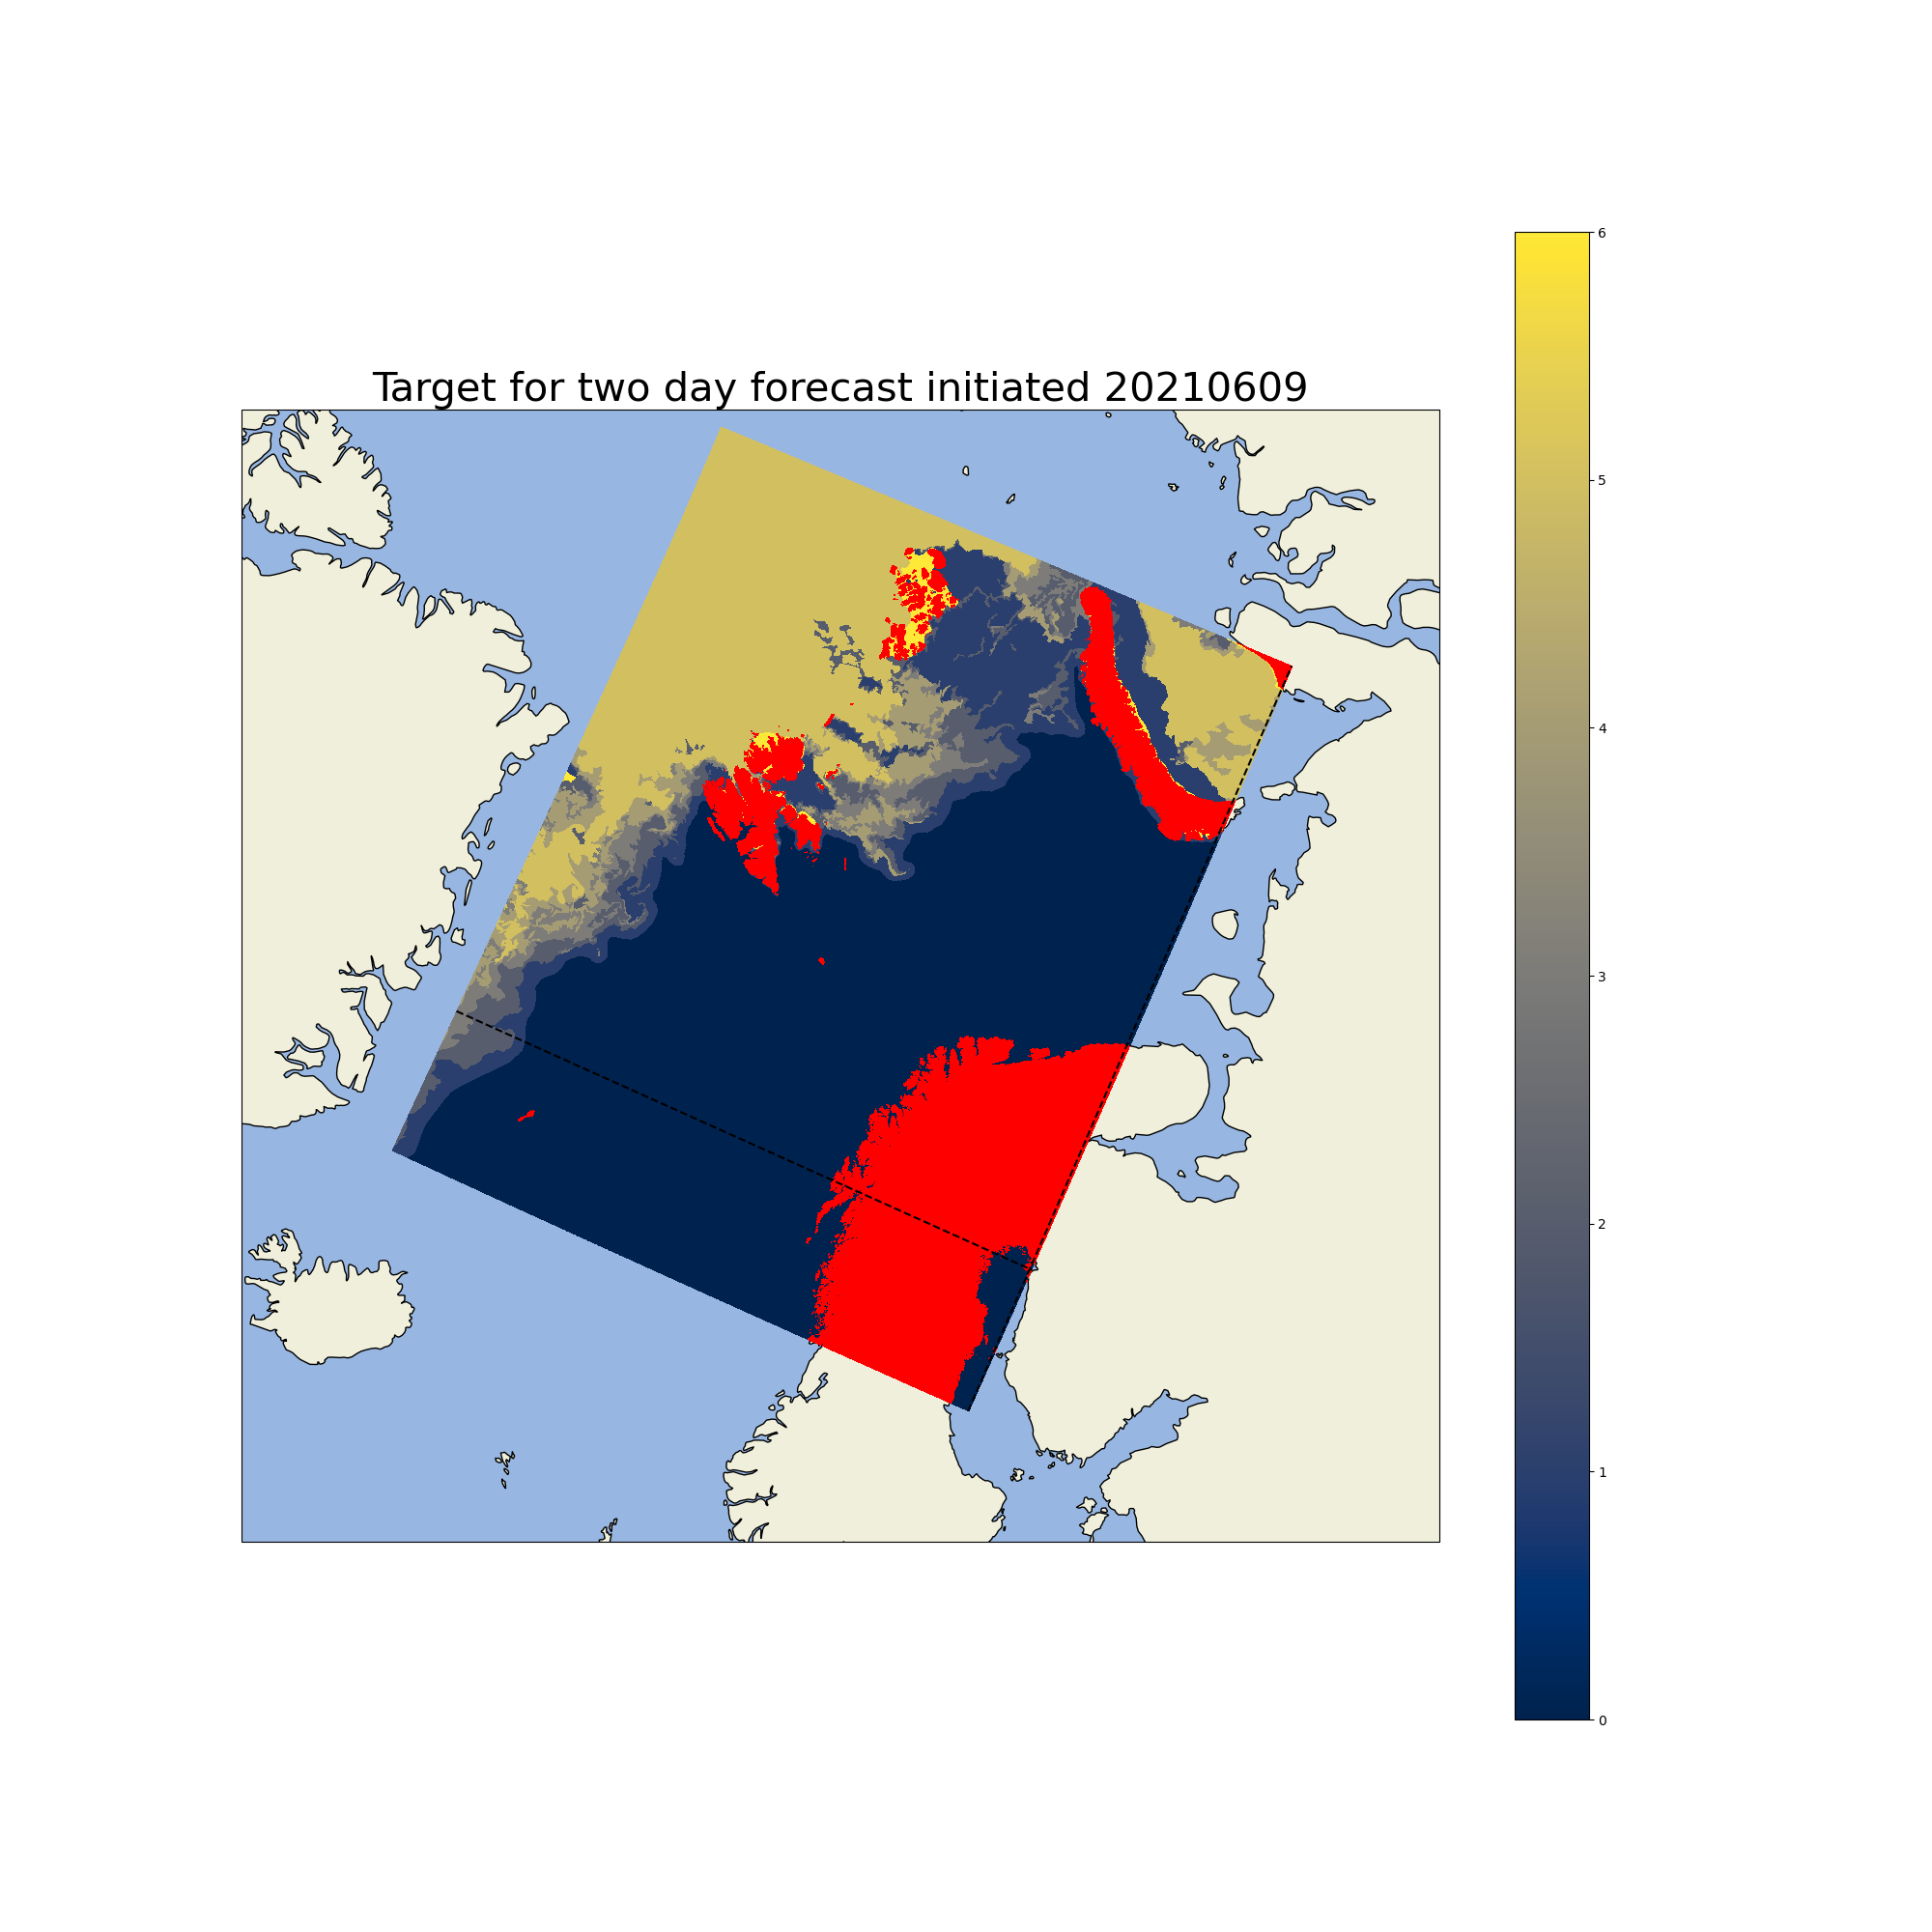
\includegraphics[trim={0 10cm 11cm 9cm}, clip, width=\textwidth]{/home/arefk/uio/MScThesis_AreKvanum2022_SeaIceML/thesis/model_development/figures/20210611_target.png}
        \caption{\label{fig:target20210611}Target for forecast with two day lead time}
    \end{subfigure}
       \caption{\label{fig:20210611}Example forecast attempt made by model\_512 and model\_1024 09-06-2021}
\end{figure}

By inspecting Figure (\ref{fig:20210611}), two observations can be made. The first observation is regarding how the model complexity affects how it fit to the data. By comparing Figure (\ref{fig:model51220210611}) with (\ref{fig:model102420210611}), it can be seen that the latter is resolving the finer structures of the ice edge to larger extent than the prior. Though the overall correctness is left to be discovered, this shows that increasing the depth of the encoder (increasing the trainable parameter count from ~7 million to ~31 million) is reflected by the model preserving the details of the ice edge structure. Though it is non-trivial to say why the 1024-model preserves the details to a larger extent than the 512-model, it does follow from the U-Net architecture that a deeper encoder (higher channel count and more convolutional blocks) is better at describing "WHAT" is in the image compared to the shallow-layers, which include a larger amount of spatial information and tells the model to a larger extent "WHERE" things are in the model. \todo{This may have a source}

The second observation made from inspecting both forecasts is their inability to represent classes 2 and 3. This likely arises from the general movement-pattern of the sea ice, where the intermediate classes are much less likely to appear than the edge-most classes. Furthermore, the sea ice is much more likely to represent a wider range of concentration classes in the intermediate ice edge region over time, making it more difficult for the network to confidently predict those classes compared to the more probable classes. As can be seen by the network immediately predicting class 4 after class 1, creating an artificial cut-off region. However, to what extent the intermediate classes are predicted has not been inspected directly \todo{They should be}, though it is likely to assume that they are predicted though with a lower confidence than that of class 4 (which is consequently why it is visualized, as the most probable class is chosen regardless).



\subsection{FocalLoss}
\todo{Include figure showing focal loss output, discuss implications of using this loss function}
The focal loss is derived as a generalization of the Cross Entropy Loss listed in Equation (\ref{eq:CE}). The intent of the loss function is to downweight the easy to predict samples, while focusing on the hard to predict samples by allowing their gradient to have a higher impact on the network \cite{Lin2017}. Mathematically, focal loss is defined as

\begin{equation}
    \label{eq:FL}
    \text{FL} = -\sum_i^C\alpha_i(1 - \hat{y}_i)^\gamma y_i\log{(\hat{y}_i)}
\end{equation}

where $\alpha$ is a balancing parameter, $\gamma$ is the focusing parameter ($\gamma = 0 \rightarrow CE$), with the rest similar as Equation (\ref{eq:CE}).

By inspecting Equation (\ref{eq:FL}), it can be seen that predictions that the model is quite confident in making, i.e. $\hat{y}_i \rightarrow 1$ send the Focal Loss towards zero. For the current application, the assumptive motivation is that this affects (by reducing) the contribution made by the Ice Free Open Water pixels as well as the Very Close Drift Ice (class 6), which are the most represented classes in the CE loss model seen in Figure (\ref{fig:20210611}). Consequently, as the loss contributions of the most likely (and most represented classes) is reduced, the harder to predict (both due to being less represented and due to sea ice movement) have a larger impact on the overall loss propagating backwards throughout the model. As a result, these intermediate classes should be predicted as the most likely class, resulting in a less sharp ice edge which closer represent the Ice Charts. 


\subsection{Cumulative probability distribution model}
\todo{Discuss difference in dataloader, same dataset is used differently}

\subsubsection{Separate convolutionial layers as output}
\todo{Data exists, start writing}

\subsubsection{Single convolutional layer for multiple outputs}
\todo{Not started on}


\biblio
\end{document}